\documentclass[12pt]{beamer}
\usepackage{xcolor}
\usepackage{tabularray}
\usepackage{caption}
\usepackage{subcaption}
\usepackage{tabularx}
\usepackage{graphics}
\usepackage{graphicx}
\usepackage{tikz}
\title{Horseback adventure}
\subtitle{“Horses teach us to fly without wings and to run without fatigue.”}
%\titlegraphic{\includegraphics{\includegraphics[scale=0.2]{logo.png}}}
\titlegraphic{
\includegraphics[scale=0.2]{logo.png}}
\author{Embark on unforgettable journeys with us—your adventure starts here!}
\date{}

\setbeamertemplate{frametitle}{
	\vspace{1em} % Adjust the vertical space
	\begin{center}
		\color{black}\textbf{\insertframetitle}\\
		\vspace*{-15pt} % Make title bold and black
		\noindent\rule{\linewidth}{1pt} % Add a horizontal line
	\end{center}
}

\setbeamerfont{footnote}{size=\scriptsize} 
\setbeamertemplate{navigation symbols}{}


\begin{document}
	\begin{frame}
		\begin{center}
			{\LARGE\textbf{\inserttitle}}\\
			\vspace*{2mm}
			{\itshape \insertsubtitle}\\
			\vspace*{2mm}
			{\inserttitlegraphic}\\
			\vspace*{2mm}
			{\textbf{\insertauthor}}
		\end{center}
	\end{frame}
	\begin{frame}
		\frametitle{3 to 4 hour horseback adventure}

				\begin{figure}
				\centering
				\subcaptionbox{first stop\footnote{The Temple of the Moon and the Sun is an ancient site with rich history and cultural significance.}}
				{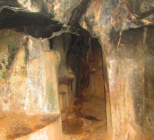
\includegraphics[scale=0.45]{1.jpg}}
				\subcaptionbox{second stop\footnote{Inkilltambo is a significant archaeological site known for its terraces, irrigation channels, and ceremonial spaces.}}
				{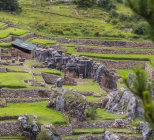
\includegraphics[scale=0.45]{2.jpg}}
				\subcaptionbox{third stop\footnote{Chuspiyoq is known for its unique carved stones and the panoramic views it offers of the surrounding landscape.}}
				{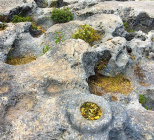
\includegraphics[scale=0.45]{3.jpg}}
				\caption{Explore ancient sites and stunning views on this horseback adventure.}
				\end{figure}

	\end{frame}
	
	\begin{frame}
		\frametitle{Half-day horseback adventure}
		    \setcounter{footnote}{0}
			
			\begin{figure}
				\centering
				\subcaptionbox{Katunqui\footnote{Apu Katunki offers a unique cultural experience and stunning landscapes. Join us to explore Andean traditions and natural beauty.}}
				{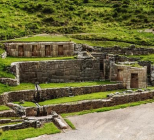
\includegraphics[scale=0.45]{4.jpg}}
				\subcaptionbox{camelids\footnote{Graze among the camelids and share the Andean culture on the spot.}}
				{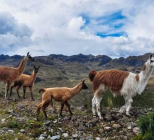
\includegraphics[scale=0.45]{5.jpg}}
				\subcaptionbox{Gallop\footnote{Enjoy the thrill of galloping and trotting through the beautiful Andean landscape.}}
				{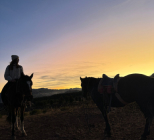
\includegraphics[scale=0.45]{6.jpg}}
				\caption{Experience Andean culture and landscapes on horseback, from cultural sites to thrilling gallops.}
			\end{figure}
			
	\end{frame}
	
	\begin{frame}
		\frametitle{Full day horseback adventure}
        \setcounter{footnote}{0}
		
		\begin{figure}
			\centering
			\subcaptionbox{Yanaqocha\footnote{Yanaqocha is the first lagoon you arrive at on horseback. The surrounding area is inhabited by people who breed llamas and alpacas, offering an authentic Andean experience.}}
			{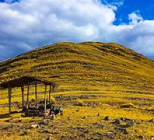
\includegraphics[scale=0.45]{7.jpg}}
			\subcaptionbox{L. Qenqo\footnote{The Qeullaqocha lagoon in the town of Qenqo is a serene spot for fishing and cooking your catch amidst the mountain scenery.}}
			{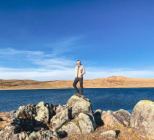
\includegraphics[scale=0.45]{8.jpg}}
			\subcaptionbox{H. Qosqo\footnote{Huchuy Qosqo is a vast archaeological site comparable to Sacsayhuamán, though less known due to its hilltop location.}}
			{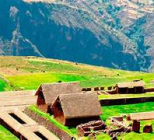
\includegraphics[scale=0.45]{9.jpg}}
			\caption{Explore Andean culture and landscapes on horseback: Yanaqocha's llama and alpaca breeders, fishing at Qeullaqocha lagoon, and the vast Huchuy Qosqo site.}
		\end{figure}
		
	\end{frame}
	
	\begin{frame}
		\frametitle{Pre-Ride Briefing and Preparation}
       \setcounter{footnote}{0}
		
		\begin{figure}
			\centering
			\subcaptionbox{Helmet\footnote{Safety helmets are provided for protection during the ride.}}
			{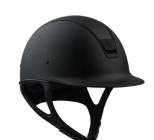
\includegraphics[scale=0.45]{10.jpg}}
			\subcaptionbox{Water\footnote{Mineral water is provided throughout the journey to keep you hydrated.}}
			{
\includegraphics[scale=0.45]{11.jpg}}
			\subcaptionbox{Gloves\footnote{Gloves are provided for a better grip and comfort while riding.}}
			{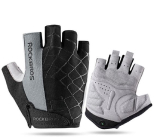
\includegraphics[scale=0.45]{12.jpg}}
			\caption{Safety and comfort: Helmets, mineral water, and gloves are provided for an enjoyable horseback riding experience.}
		\end{figure}
	\end{frame}
	
	\begin{frame}
			\begin{center}
				{\Large\itshape
					May the rhythm of the horse's hooves and the beauty of the Andean landscapes leave footprints on your heart.\\
					Until we ride together again.
				}
			\end{center}
	\end{frame}
	
	
\end{document}